% This is Deliverable 1 of Project 2

\documentclass[12pt]{article}
\usepackage{amsmath}
\usepackage{amssymb}
\usepackage{fancyhdr}
\usepackage{geometry}
\usepackage{hanging}
\usepackage{enumitem}
\usepackage{graphicx}
\usepackage{setspace}
\usepackage{tabularx}
\usepackage{array}
\usepackage{xcolor}
\usepackage{longtable}
%\usepackage{lipsum} %remove later
\doublespacing
%\setlength\parindent{28 pt}
\geometry{letterpaper, margin=1in}

% ++++ Fancy Settings (for header) ++++
\pagestyle{plain}
\fancypagestyle{main}{
	\fancyhf{}
	\lhead{Assessment Report}
	\rhead{\leftmark}
	\cfoot{\thepage}
	\renewcommand{\headrulewidth}{0.4pt}
}

% Column widths (tweak the numbers if you want)
\newcommand{\colNum}{0.06\linewidth}   % column 1 (1–10)
\newcommand{\colSmall}{0.16\linewidth} % columns 2,3,5
\newcommand{\colMed}{0.25\linewidth}
\newcommand{\colBig}{0.48\linewidth}   % column 4 (3x colSmall)

% ++++ Begin Doc ++++

\begin{document}

% ++++ Cover Page ++++

\begin{titlepage}
\centering
\vfill

% ++Logo

\includegraphics[width=0.35\textwidth]{images/logo.png}

\vspace{1.5cm}

% ++Title
\LARGE{\textbf{Assessment Report}}\\
\vspace{0.3cm}
\large{\textbf{Keith Schoen}}\\
\vspace{0.3cm}
\large{\textbf{CSEC3755-001}}\\
\vspace{0.3cm}
\large{\textbf{Dr. Daniel Pittman}}\\
\vspace{0.3cm}
\large{\textbf{28 April, 2026}}\\
\vspace{0.3cm}

\vfill
\end{titlepage}

% ++++ ToC ++++

\pagenumbering{gobble} %hide page numbers for cover and ToC
\tableofcontents
\clearpage

% ++++ Begin Report ++++

\pagenumbering{arabic} %page one starts here
\setcounter{page}{1}
\pagestyle{main} %turn on fancy

% ++++ P01 ++++
\section{Executive Summary} 
\subsection{Overall Security Posture: Medium}
MedTech's internal network was assessed across two primary systems — the Ubuntu application server and the Windows web server. No catastrophic or immediately exploitable vulnerabilities were found. However, several configurations that were likely never intentionally set up as permanent features have been left in place and represent real, addressable risk. The overall posture is rated Medium: the network is not on fire, but it has unlocked doors that need to be closed before someone walks through them.
\subsection{Top 5 risks requiring immediate attention}
\begin{enumerate}
	\item \textbf{A folder named "confidential" is publicly accessible with no password.} The Ubuntu server is running a file transfer service that allows anyone on the network to log in anonymously — no username, no password — and browse its contents. At the time of assessment, that included a directory explicitly named "confidential." This requires no technical skill to exploit. Anyone who can reach the network can open a file browser and start downloading. This is the single highest-priority item in the assessment.
	\item \textbf{Passwords are being sent across the network in plain text.} The Ubuntu server hosts a web application with a login page. When a user types their password and clicks submit, that password travels across the network unencrypted — readable by any device on the same network segment, the same way you can read a postcard in the mail. The same is true of the FTP file transfer service. If any of those credentials are shared with other systems, a single intercepted login could open multiple doors.
	\item \textbf{The Windows server's remote access is using outdated encryption.} The Windows server allows remote desktop connections — a standard and legitimate capability — but it is negotiating those connections using encryption standards from 2011 that have known weaknesses. Remote desktop is one of the most common entry points for ransomware attacks in healthcare environments. Updating the encryption configuration is a low-effort, high-value fix.
	\item \textbf{The Windows server is advertising its internal structure to anyone who asks.} A standard query to port 135 on the Windows machine returns a detailed map of its internal services, including its security and print management processes. This is not an attack in itself, but it is the reconnaissance step that precedes one. It tells an attacker exactly which doors exist before they try to open them.
	\item \textbf{Two systems sharing the same weak security setting on remote access.} Both the Ubuntu and Windows servers support an outdated cryptographic method for their SSH remote access channels. This is a lower-urgency item than the above four, but it applies to both machines and is a five-minute configuration fix on each.
\end{enumerate}
\subsection{Key recommendations summary}
All five issues above are configuration problems, not hardware or software purchases. Remediation does not require new products or significant capital expenditure — it requires scheduled maintenance time and the right technical hands. In order of priority:\\
First, disable anonymous access on the file transfer service and review the contents of the "confidential" directory immediately to assess whether any sensitive data has already been accessed.\\
Second, enforce encrypted connections on both the web login page and the file transfer service. This is a standard configuration change and should be bundled into a single maintenance window with the first item.\\
Third, update the Windows remote desktop service to require modern encryption only, and restrict which network addresses are permitted to initiate remote desktop sessions at all.\\
Fourth, restrict the Windows server's internal service information from being visible to the broader network. This is a firewall rule change.\\
Fifth, update the SSH configuration on both servers to remove the weak cryptographic option. Low urgency, but a clean and fast hardening item.\\
Realistically, items one through three can be addressed in a single focused maintenance window. Items four and five can follow in the next scheduled cycle. None of these require outside vendors or procurement.\\
\subsection{HIPAA compliance implications}
MedTech operates in a healthcare-adjacent environment, which means the HIPAA Security Rule is not a background consideration — it is a legal obligation with financial consequences. Two findings in this assessment have direct compliance relevance.//
The publicly accessible "confidential" directory (item 1) is a potential violation of the HIPAA Security Rule's access control standard, which requires that access to electronic protected health information be limited to authorized users only. If that directory contains or has ever contained patient data, billing records, or any information that could identify a patient, the organization may have an obligation to assess whether a reportable breach has occurred. Breach penalties under HIPAA range from \$100 to \$50,000 per violation, with an annual cap of \$1.9 million per violation category — and that is before factoring in reputational damage or legal exposure.\\
The unencrypted credential transmission findings (items 2 and 3) are a direct gap against the transmission security standard, which requires that ePHI be encrypted when transmitted over a network. Even if those specific login pages do not handle patient data directly, the standard applies to the systems that do — and a compromised credential on one system is often a path to another.\\
The practical takeaway for budgeting purposes: the cost of remediating all five items above is measured in staff hours. The cost of a HIPAA breach investigation, corrective action plan, and potential fine is measured in hundreds of thousands of dollars at minimum. The math strongly favors acting now.\\

% ++++ P02 ++++
\section{Network Topology Documentation}
\subsection{Asset Inventory}
{\singlespacing
	\begin{longtable}{
 		|| >{\raggedright\arraybackslash}p{\colSmall}
  		| >{\raggedright\arraybackslash}p{\colSmall}
  		| >{\raggedright\arraybackslash}p{\colMed}
  		| >{\raggedright\arraybackslash}p{\colMed} ||}
		\hline
		\textbf{IP} & \textbf{Hostname} & \textbf{OS} & \textbf{Role} \\
		\hline\hline
		\endhead
		192.168.56.102 & MedTech / 6C3D442378D3 & Ubuntu Linux & Application server \\
		\hline
		192.168.56.103 & kali & Kali Linux (Debian) & Scanner / attack machine \\
		\hline
		192.168.56.105 & - & Windows & IIS web server \\
		\hline
		192.168.56.106 & - & Linux Router & MedTech router / firewall \\
		\hline
	\end{longtable}
}

\subsection{Open Ports and Services Per Host}
\textbf{Ubuntu (192.168.56.102)}
\begin{itemize}
	\item \textbf{21/tcp-vsftpd (FTP)} - anonymous login enabled, \texttt{confidential} and \texttt{public} directories exposed
	\item \textbf{22/tcp} - OpenSSH 9.6p1 Ubuntu 3ubuntu13.15
	\item \textbf{25/tcp} - SMTP (MedTech Solutions SMTP Server v1.4)
	\item \textbf{80/tcp-Werkzeug httpd 2.2.0 (Python 3.9.25)} - login from transmitting credential in cleartext
	\item \textbf{139/tcp, 445/tcp} - Samba smbd 3.x-4.x (workgroup:MEDTECH)
	\item \textbf{3306/tcp} - MySQL 8.0.45
\end{itemize}
\textbf{Windows (192.168.56.105)}
\begin{itemize}
	\item \textbf{22/tcp} - OpenSSH for Windows 9.5
	\item \textbf{80/tcp} - Microsoft IIS httpd 10.0
	\item \textbf{135/tcp} - Microsoft RPC
	\item \textbf{445/tcp} - Microsoft-DS (SMB)
	\item \textbf{3389/tcp} - Microsoft Terminal Services (RDP)
	\item \textbf{5985/tcp} - Microsoft HTTPAPI 2.0 (WinRM/SSDP/UPnP)
\end{itemize}
\textbf{Router (192.168.56.106)}
\begin{itemize}
	\item \textbf{22/tcp} - OpenSSH 10.2
	\item \textbf{10000/tcp} - Webmin (MiniServ) admin panel	
\end{itemize}

\section{Vulnerability Assessment}
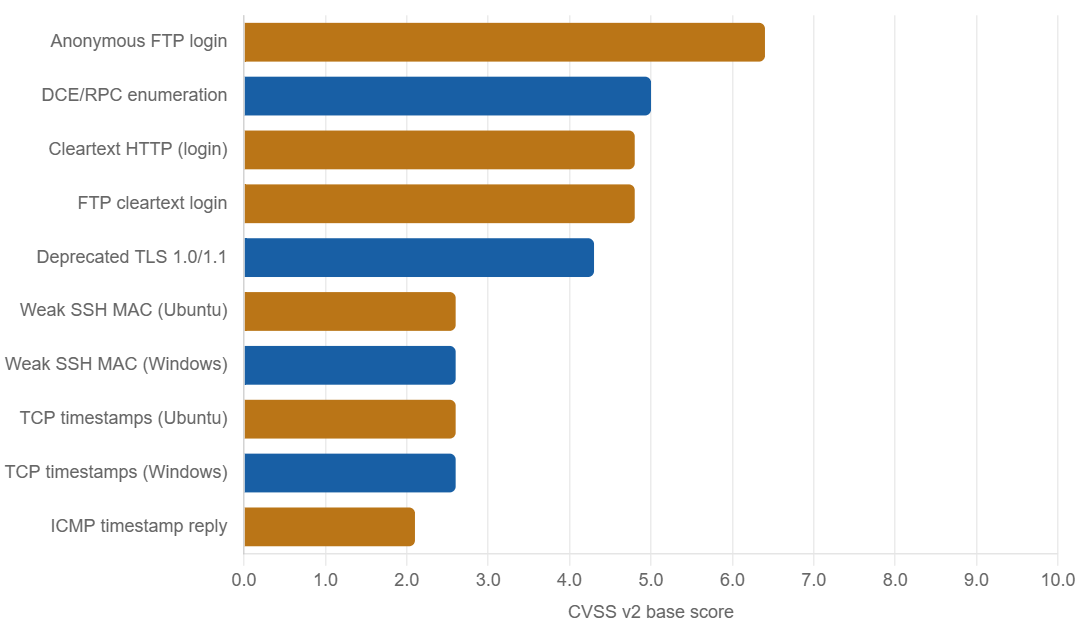
\includegraphics[width=\textwidth]{images/scan-assessment.png}\\ \textit{Figure 01: Chart created by Claude with information from reports}
\subsection{Medium Severity (CVSS 4.3-6.4)}
\begin{enumerate}
	\item \textbf{Anonymous FTP login enabled — CVSS 6.4}\\
		System: Ubuntu 192.168.56.102, port 21\\
		CVE: CVE-1999-0497\\
		The FTP server accepts both anonymous and ftp as valid usernames with no real password verification. At the time of scan, the anonymous account had access to two directories: confidential and public. That directory name alone is a significant flag for a healthcare-adjacent organization. An attacker can browse, download, and depending on permissions, upload or delete files — all without any credentials. HIPAA relevance is direct: if the confidential directory contains any patient records, billing data, or PHI of any kind, this is a potential reportable breach vector under the HIPAA Security Rule (45 CFR §164.312), which requires access controls ensuring only authorized users reach ePHI.
	\item \textbf{DCE/RPC and MSRPC services enumeration — CVSS 5.0}\\
		System: Windows 192.168.56.105, port 135\\
		No CVE assigned.\\
		Windows RPC endpoint mapper on port 135 is responding to enumeration queries and disclosing a full list of active RPC services, including lsass.exe (SAM access / Local Security Authority), spoolsv.exe (Print Spooler), and Windows Event Log endpoints. This is an information disclosure finding — an attacker uses this map to identify which services to target for privilege escalation or lateral movement. The Spooler service in particular has a long history of critical exploits (e.g., PrintNightmare). HIPAA relevance is indirect but real: this enumeration is typically a precursor step in a targeted attack chain against a Windows host storing or processing ePHI.
	\item \textbf{Cleartext HTTP transmission of credentials — CVSS 4.8}\\
		System: Ubuntu 192.168.56.102, port 80\\
		No CVE assigned (references CWE-319).\\
		The web application at http://192.168.56.102/login accepts a password field over plain HTTP with no TLS. Any credentials submitted are transmitted unencrypted and can be intercepted by anyone on the network segment via a passive man-in-the-middle attack. Given that the Ubuntu machine is running Samba, MySQL, and SMTP — all of which may share credentials — compromise of the web login could cascade. HIPAA relevance: the Security Rule's transmission security standard (45 CFR §164.312(e)(1)) requires encryption of ePHI in transit. An unencrypted login page on a clinical or administrative system would be a direct violation.
	\item \textbf{FTP cleartext login — CVSS 4.8}\\
		System: Ubuntu 192.168.56.102, port 21\\
		No CVE assigned.\\
		Separate from the anonymous login finding, the FTP service also accepts authenticated (non-anonymous) logins without requiring AUTH TLS first. This means any user's FTP credentials are transmitted in plaintext. Same transmission security concern as finding \#3, but compounded because FTP credentials may be reused across other services on the host. HIPAA relevance mirrors finding \#3.
	\item \textbf{Deprecated TLS 1.0 and 1.1 protocols — CVSS 4.3}\\
		System: Windows 192.168.56.105, port 3389 (RDP)\\
		CVEs: CVE-2011-3389 (BEAST), CVE-2015-0204 (FREAK)\\
		The RDP service is advertising support for TLS 1.0 and 1.1 in addition to TLS 1.2+. Both older protocol versions have known cryptographic weaknesses that can allow an attacker to downgrade the connection and potentially decrypt traffic. RDP carrying deprecated TLS is particularly sensitive because RDP sessions on a Windows server likely include administrative access and potentially PHI-handling workflows. HIPAA relevance: same transmission security standard as above, and RDP itself is one of the most commonly exploited remote access vectors in healthcare ransomware attacks.
	\end{enumerate}
\subsection{Low Severity (CVSS 2.1-2.6)}
\begin{enumerate}
	\item[6.~7.] \textbf{Weak SSH MAC algorithms — CVSS 2.6}\\
		Systems: Both Ubuntu (.102, port 22) and Windows (.105, port 22)\\
		Both SSH servers advertise support for umac-64-etm@openssh.com and umac-64@openssh.com — 64-bit MAC algorithms considered cryptographically weak by current standards. An attacker with the ability to capture SSH session traffic could theoretically exploit this, though it requires significant capability. Low priority but a clean hardening item.
	\item[8.~9.] \textbf{TCP timestamps information disclosure — CVSS 2.6}\\
		Systems: Both Ubuntu (.102) and Windows (.105)\\
		Both hosts implement RFC1323 TCP timestamps, allowing an attacker to estimate system uptime. Uptime data can narrow the window of unpatched vulnerabilities (e.g., "this system hasn't rebooted in 90 days, so patches applied in that period are unapplied"). Negligible standalone risk but contributes to an attacker's reconnaissance picture.
	\item[10] \textbf{ICMP timestamp reply — CVSS 2.1}\\
		System: Ubuntu 192.168.56.102\\
		CVE: CVE-1999-0524\\
		The host responds to ICMP Type 13 (timestamp) requests, disclosing system clock information. Theoretical risk to time-based random number generation in other services. Lowest-priority finding in the assessment.
\end{enumerate}
\section{Risk Prioritization}
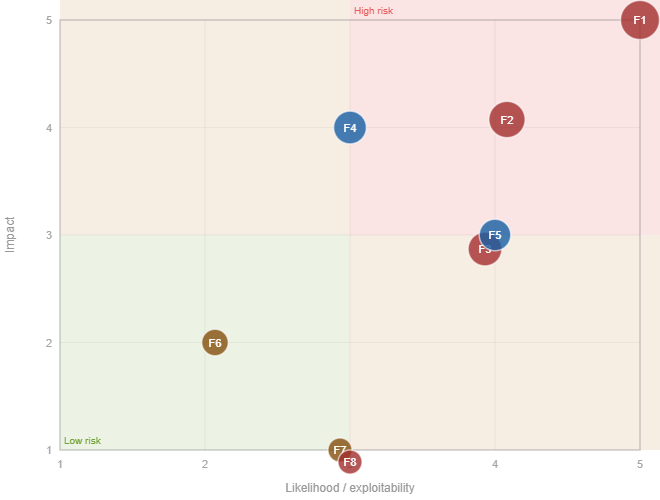
\includegraphics[width=\textwidth]{images/risk-matrix.png}\\ \textit{Figure 02: Matrix created by Claude with information from reports}
\begin{table}[h]
\centering
\renewcommand{\arraystretch}{1.3}
\resizebox{\textwidth}{!}{
\begin{tabular}{|c|l|c|c|c|c|c|c|}
\hline
\textbf{ID} & \textbf{Finding} & \textbf{Exploit.} & \textbf{Impact} & \textbf{Asset Val.} & \textbf{HIPAA} & \textbf{Composite} & \textbf{Priority} \\
\hline
F1 & Anonymous FTP login         & 5 & 5 & 5 & 5 & \textbf{5.00} & 1 \\
F2 & Cleartext HTTP credentials  & 4 & 4 & 5 & 5 & \textbf{4.45} & 2 \\
F3 & FTP cleartext login         & 4 & 3 & 5 & 4 & \textbf{3.95} & 3 \\
F4 & Deprecated TLS on RDP       & 3 & 4 & 4 & 4 & \textbf{3.75} & 4 \\
F5 & DCE/RPC enumeration         & 4 & 3 & 4 & 3 & \textbf{3.45} & 5 \\
F6 & Weak SSH MAC algorithms     & 2 & 2 & 4 & 2 & \textbf{2.50} & 6 \\
F7 & TCP timestamp disclosure    & 3 & 1 & 3 & 1 & \textbf{1.95} & 7 \\
F8 & ICMP timestamp reply        & 3 & 1 & 3 & 1 & \textbf{1.95} & 8 \\
\hline
\end{tabular}
}
\textit{Composite $=$ exploitability$\times$0.25 $+$ impact$\times$0.30 $+$ asset value$\times$0.25 $+$ HIPAA$\times$0.20}
\label{tab:risk-matrix}
\end{table}
\subsection{Prioritization}
\begin{enumerate}
	\item \textbf{Disable anonymous FTP (F1)} Fix immediately. This is the single highest-risk finding in the assessment. A directory named confidential is accessible to anyone with a network connection and a basic FTP client — no exploit required. Until this is closed, every other control on the Ubuntu machine is undermined. Remediation: disable anonymous login in /etc/vsftpd.conf (anonymous\underbar{   }enable=NO), or disable FTP entirely and replace with SFTP if file transfer is required at all. Effort is minimal; the risk of inaction is severe.
	\item \textbf{Enforce HTTPS on the web application (F2)} Fix immediately alongside F1. Credentials submitted to http://192.168.56.102/login are readable in plaintext by any host on the subnet. The Werkzeug development server in use is also a red flag — Werkzeug is a Python debugging framework, not a production web server, and it should never be internet- or network-facing. Remediation: deploy a TLS certificate and force HTTPS redirects; replace Werkzeug with a production WSGI server (nginx + gunicorn) for any real deployment.
	\item \textbf{Enforce FTPS or migrate to SFTP (F3)} Fix in the same maintenance window as F1/F2. The FTP service accepting authenticated sessions over cleartext is a compounding risk — if anonymous access is removed but cleartext auth remains, credential exposure persists. Remediation: enable AUTH TLS enforcement in vsftpd, or migrate file transfer entirely to SFTP over the existing SSH service, eliminating FTP altogether.
	\item \textbf{Disable TLS 1.0 and 1.1 on RDP (F4)} Schedule within the next patch cycle. RDP with deprecated TLS is particularly dangerous for a healthcare-adjacent host because RDP is the most common ransomware entry vector in healthcare incidents. Disabling older protocols is a one-time registry change on Windows. Remediation: set \verb|HKLM\SYSTEM\CurrentControlSet\Control\SecurityProviders\SCHANNEL\Protocols| to disable TLS 1.0 and 1.1, or apply via Group Policy. Consider whether RDP needs to be open on the network-facing interface at all.
	\item \textbf{Restrict RPC endpoint exposure (F5)} Address during the same Windows hardening pass as F4. Port 135 should not be reachable from untrusted network segments. The Spooler and LSASS RPC endpoints it exposes are well-documented attack targets. Remediation: firewall rules restricting port 135 to trusted management addresses only; disable the Print Spooler service if printing is not required on this host.
	\item \textbf{Harden SSH MAC configuration (F6)} Low urgency but a clean hardening item for both hosts. Remediation: add MACs hmac-sha2-256,hmac-sha2-512 to /etc/ssh/sshd\underbar{   }config on Ubuntu and the equivalent OpenSSH for Windows config, then restart the SSH service. Five-minute fix on each host.
	\item[7.~8.] \textbf{Suppress TCP and ICMP timestamps (F7, F8)} Address opportunistically during next scheduled maintenance. These are genuine hardening items but pose negligible standalone risk. Remediation for Ubuntu: add net.ipv4.tcp\underbar{   }timestamps=0 to /etc/sysctl.conf and run sysctl -p; block ICMP Type 13 at the firewall. On Windows: netsh int tcp set global timestamps=disabled (with the caveat that Windows Server 2008+ cannot fully disable TCP timestamps when the peer initiates them).
\end{enumerate}

\vfill
\textit{++report written with help from Claude (Sonnet 4.6)++}
\end{document}

% +++++++++ Helpful stuff +++++++++++
%
% +++ Using Minipages +++
% \begin{minipage}[t]{\linewidth}
% \includegraphics[width=0.50\textwidth]{*Image file}\\
% \textit{*Image subtitle}
% \end{minipage}
% \end{enumerate}
%


% +++ Fixed width table +++
%\begin{tabularx}{1.0\textwidth}{
%	|| >{\raggedright\arraybackslash}X
%	|  >{\raggedright\arraybackslash}X
%	|  >{\raggedright\arraybackslash}X
%	|  >{\raggedright\arraybackslash}X || }
%	\hline
%	\textbf{x} & \textbf{x} & \textbf{x} & \textbf{x} \\
%	\hline \hline
%	x $ x $ x & x & x & x  \\
%	\hline
%	x $ x $ x & x & x & x \\
%	\hline
%	x $ x $ x & x & x & x \\
%	\hline
%	x $ x $ x & x &  x  & x \\
%	\hline
%\end{tabularx}
%

% +++ For tables that take multiple pages +++
%{\singlespacing
%	\begin{longtable}{
% 		|| >{\centering\arraybackslash}p{\colNum}
%  		| >{\raggedright\arraybackslash}p{\colSmall}
%  		| >{\raggedright\arraybackslash}p{\colSmall}
%  		| >{\raggedright\arraybackslash}p{\colBig}
%  		| >{\raggedright\arraybackslash}p{\colSmall} ||}
%		\hline
%		\textbf{x} & \textbf{x} & \textbf{x} & \textbf{x} & \textbf{x} \\
%		\hline\hline
%		\endhead
%		\hline
%  	    	 x & x & x & x  & x \\
%		\hline
%	\end{longtable}
%}












